\documentclass[../main.tex]{subfiles}
\begin{document}
%\chapter{Finto}
%\chapter{Finto}
%\newpage
\setchapterstyle{kao}
\setchapterpreamble[u]{\margintoc}
\chapter[Tangent and cotangent spaces]{Tangent and cotangent spaces}
\labch{tang_space}
\section{Tangent vectors}
\underline{Question:} How do we define tangent vector to a manifold $\mathbf{M}$ \underline{\textbf{intrinsically}}?? There are two viewpoint on this, both interesting, we will see first the \textit{geometric viewpoint}, which is the one the professor likes more, and the the algebraic one. We will not prove the equivalence of the two viewpoints, but we will say few words on that.
\begin{marginfigure}[20mm]
	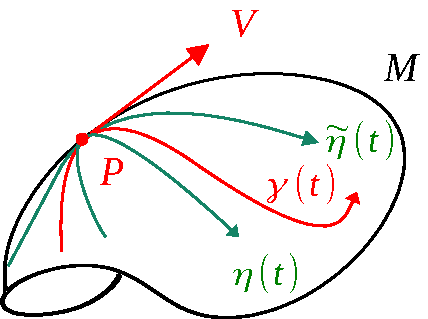
\includegraphics{images/tan_int.pdf}
	\caption[Representatio of a tangent vector.]{Representation of a tangent vector to a point $P$ associated to a curve $\gamma$. The curves $\eta$ and $\Tilde{\eta}$ have the same tangent vector.}
	\labfig{tan-int}
\end{marginfigure} 
\subsection[Geometric viewpoint]{Geometric viewpoint}
So would like to define the vector $V$ in \reffig{tan-int}, which does not exist as we represented in the same figure since it needs an embedding space. If $\mathbf{M} \subseteq \mathbb{R}^n$, every tangent vector is the \textbf{"velocity"} of a smooth curve
\[
\begin{split}
\gamma : (-\varepsilon,+\varepsilon)& \xrightarrow[]{C^\infty} \mathbf{M}\\
t &\mapsto \gamma(t)
\end{split}
\] with $\gamma(0)=P$ such that $\Dot{\gamma}(0)=V$. We could identify $V$ with the corresponding $\gamma$, but there might exist different curves with the same tangent vector $V$: $\Dot{\gamma}(0)=V=\Dot{\eta}(0)$ (\reffig{tan-int}) with a one to infinity correspondence ({\fontencoding{U}\fontfamily{futs}\selectfont\char 66\relax} redundancy). In mathematics, when this happens, it means that we need to introduce quotients in order to define equivalent relations. We have to \textbf{identify curves with the same tangent vector}. How? Obviously, \todo{From this point, \textbf{no embedding} anymore}\textbf{in the local charts!} 
\begin{figure}[H]
	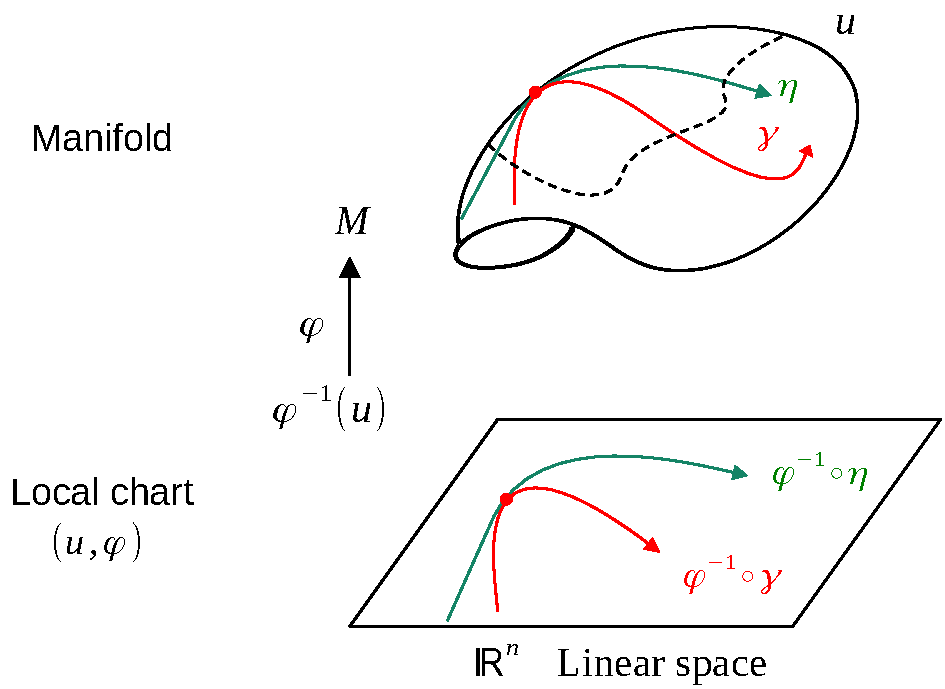
\includegraphics{images/tan_equiv.pdf}
	\caption[Tangential equivalence]{Representation of the tangential equivalence between two maps.}
	\labfig{tan-equiv}
\end{figure} 
\begin{definition}[Tangential equivalence]\index{Tangential equivalence}
Let $\mathbf{M}$ be a (smooth) manifold and $P \in \mathbf{M}$. Define\footnote{To be very precise, we should specify that the $\varepsilon$ depends on $\gamma$ by writing $\varepsilon \to \varepsilon_\gamma$.}
\[
K_P(\mathbb{M})=\left\{\gamma:(-\varepsilon,+\varepsilon)\xrightarrow[]{C^\infty}\mathbf{M}:\varepsilon>0, \gamma(0)=P \right\}
\]
We say that $\gamma$ and $\eta$ are \textbf{tangentially equivalent} in $K_P(\mathbf{M})$ if in a local chart $(u,\varphi)$ [and, henche, in all local charts] it happens that $P \in u$ and
\[
\dv{t}(\varphi^{-1}\circ \gamma)\Bigr|_{\substack{t=0}}=\dv{t}(\varphi^{-1}\circ \eta)\Bigr|_{\substack{t=0}}
\]
\end{definition}
i.e. if $\varphi^{-1} \circ \gamma$ and $\varphi^{-1} \circ \eta$ have the same tangent vector in $\varphi^{-1}(u)\subseteq\mathbb{R}^n$.
%\begin{marginfigure}
%	\includesvg[width=1.3\linewidth]{images/Tangentialvektor.svg}
%	\caption[Tangent space]{From \href{https://it.wikipedia.org/wiki/Spazio_tangente}{Wikipedia}: The tangent space $T_{x}M$ and a tangent vector $v\in T_{x}M$, along a curve traveling through $x\in M$.}
%	\labfig{tan-space}
%\end{marginfigure} 
\begin{definition}[Tangent vector]\index{Tangent vector}
A \textbf{tangent vector} $V$ at the point $P\in\mathbf{M}$ is an equivalence class of \textbf{tangentially equivalent curves in} $K_P(\mathbf{M})$, namely $V=[\gamma]$.
\end{definition}
\begin{definition}[Tangent space]
The tangent space at $P\in\mathbf{M}$ is defined as
\[
T_P\mathbf{M}=K_P(\mathbf{M})\big/ \underset{\mathclap{\tikz \node {$\uparrow$} node [below=1ex] {\footnotesize Tangential equivalence};}}{\sim} \ =\{[\gamma]:\gamma\in K_P(\mathbf{M})\} \qquad \star
\]
\end{definition}
\begin{example}(easy)
Prove that if two curves $\gamma, \eta$ in $K_P(\mathbf{M})$ are tangentially equivalent, then they are equivalent in any other chart $(\tilde{u},\tilde{\varphi})$ in the atlas.
\end{example}
\subsection{Coordinate basis}
\begin{marginfigure}
	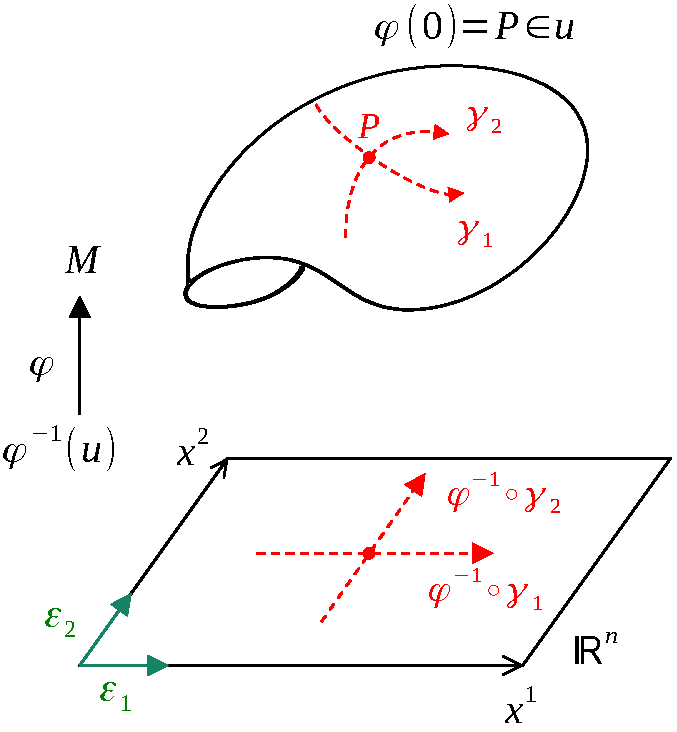
\includegraphics[width=1.3\linewidth]{images/coord_basis.pdf}
	\caption[Coordinate bases]{Picture of a manifold and a local chart in $\mathbb{R}^2$. The convection is to write the index of the local coordinates upstairs. The pair $\varepsilon_{1,2}$ are the vectors of the canonical bases.}
	\labfig{coord-bases}
\end{marginfigure} 
Take a manifold and fix a local chart in $\mathbb{R}^n$ as in \reffig{coord-bases} and take a point $P\in u$. If we take two lines, their preimage will be two lines on the local chart. 
\[
\textrm{\underline{Ex:} Meridians and parallels on the Earth's surface}
\]
\begin{definition}[Coordinate curves]\index{Coordinate curves}
Define the \textbf{coordinate curves} for $j \in \{1,2,\dots,n\}$:
\[
\gamma_j(t)=\varphi(x_0+t\varepsilon_j)\in\mathbf{M}
\]
obviously \(\gamma_j\in K_P(\mathbf{M})\)
\end{definition}
\begin{definition}[Coordinate basis]\index{Coordinate basis}
The \textbf{coordinate basis} associated to a local chart $(u,\varphi)$ is the family $\{e_1,e_2,\dots,e_n\}\subseteq T_P\mathbf{M}$ with\marginnote{
\begin{kaobox}[frametitle=Notation]
As a notational shortcut, we will write \(\Dot{\gamma}(0)\equiv \qty[\gamma]\). It is a notation that reminds the case of the embedding.
\end{kaobox}
}\
\[
e_j\Bigr|_{\substack{P}}=[\underset{\mathclap{\tikz \node {$\uparrow$} node [below=1ex] {\footnotesize j-th coordinate in $(u,\varphi)$};}}{\gamma_j}]\equiv\Dot{\gamma_j}(0)\in T_P \mathbf{M}
\]
\end{definition}
\subsection{Linear structure}
To realize that the tangent space is a linear or vector space\sidenote{"For us Linear space" and "Vector space" are absolute synonymous.}, we have to give a linear structure to it.
\begin{definition}[Linear space]\index{Linear space}\index{Vector space}
$T_P\mathbf{M}$ is a \textbf{linear space} (= \textbf{vector space}) when equipped with the following operations: if $V=[\gamma]$ and $W=[\eta]$ are vectors in $T_P\mathbf{M}$ and $\lambda\in\mathbb{R}$, we define:\marginnote{The terms between $\big[\ \big]$ are equivalent classes in $K_P(\mathbf{M})\big/\sim$.}
\[
\begin{split}
V\overset{\mathclap{\tikz \node {$\downarrow$} node [above=1ex] {\footnotesize in $T_P\mathbf{M}$};}}{+}W&:=\Big[\varphi\big(\varphi^{-1}(\gamma)\overset{\mathclap{\tikz \node {$\downarrow$} node [above=1ex] {\footnotesize in $\mathbb{R}^n$};}}{+}\varphi^{-1}(\eta)\big)\Big]\\
\lambda V&:=\Big[\varphi\big(\lambda \underset{\mathclap{\tikz \node {$\uparrow$} node [below=1ex] {\footnotesize in $\mathbb{R}^n$};}}{\cdot} \varphi^{-1}(\gamma)\big)\Big]
\end{split}
\]
$(T_P\mathbf{M},+,\cdot)$ is a linear space.\footnote{We will not prove this because this is not a course of mathematics.}
\end{definition}
It happens that the coordinated bases is a linear bases for this vector space. So, any vector $v=[\gamma]\in T_P\mathbf{M}$ can be decomposed uniquely on the coordinate basis\marginnote{We write the vectors using capital latin letters and its component using the lowercase ones.}
\[
V=\sum_{j=1}^n \underset{\mathclap{\tikz \node {$\uparrow$} node [below=1ex] {\footnotesize components of $V$ in the coordinate space};}}{v^j} e_j
\]
We face again the usual fact of differential geometry: <<Nomina non sunt essentia rerum>>
\[
\text{\parbox{3.125 cm}{\centering coordinates in $(\tilde{u},\tilde{\varphi})$\\[-1pt]  $(\tilde{v_1},\dots,\tilde{v_n})$}} \longleftarrow {\parbox{2.5 cm}{\centering intrinsic object\\[-1pt]  $V \in T_P\mathbf{M}$}} \longrightarrow {\text{\parbox{3.125 cm}{\centering coordinates in $(u,\varphi)$ \\[-1pt] $(v_1,\dots,v_n$)}}}
\]
How are they related? By the \textbf{Jacobian matrix} of the \textbf{change of coordinates} but... which one? We emphasized in \vrefdef{comp-charts} that there are two change of coordinates, as represented in the memo on \reffig{Memo-Coordinate-transformation} that is here re-proposed. 
\begin{marginfigure}
	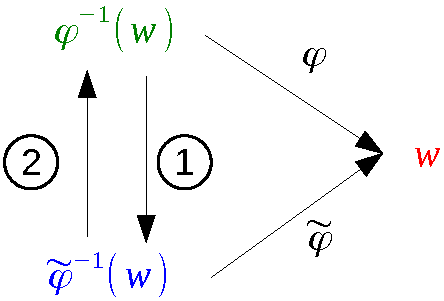
\includegraphics{images/memo_trasf.pdf}
	\caption*{Memo for the coordinate transformation}
	\labfig{Memo-Coordinate-transformation2}
\end{marginfigure} 
This is the point where the Ricci's calculus helps us, and the fact of writing indices either as subscripts or as superscripts will help us a lot thanks to the Ricci's rule\index{Ricci's rule} which states:
\[
\mbox{Ricci's rule:  "the \underline{tilde} \underline{follows} the index"
} \ \Big|\Big|
\]
We will skip the justification of this rule, but all the \href{https://en.wikipedia.org/wiki/Ricci_calculus}{Ricci's calculus} is designed to make this rule true. The index is up, the tilde is upstairs
\[
\tilde{v}^{\textcolor{red}{j}}=\sum_{l=1}^n\underbrace{\frac{\partial\textcolor{red}{\tilde{x}^j}}{\partial x^l}}_{\mathclap{\text{Jacobian matrix of the transformation $\tilde{x}(x)$}}}v^l
\]
The index is down, the tilde is downstairs
\begin{marginfigure}
	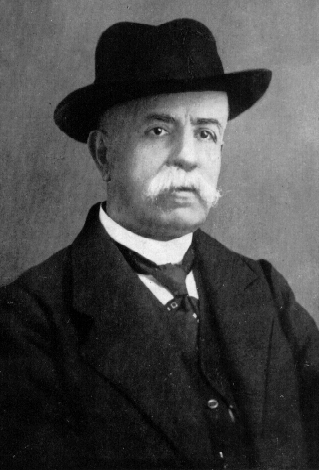
\includegraphics[width=1\linewidth]{images/Ricci_Curbastro_(cropped).jpg}
	\caption[Photo of Gregorio Ricci Cubastro]{From \href{https://commons.wikimedia.org/wiki/File:Ricci_Curbastro_(cropped).jpg}{Wikimedia}: Gregorio Ricci-Curbastro (12 January 1853 – 6 August 1925) was an Italian mathematician. He is most famous as the inventor of tensor calculus. With his former student Tullio Levi-Civita, he wrote his most famous single publication, a pioneering work on the calculus of tensors, signing it as Gregorio Ricci. This appears to be the only time that Ricci-Curbastro used the shortened form of his name in a publication, and continues to cause confusion.}
	\labfig{Ricci}
\end{marginfigure}
\[
\tilde{e}_{\textcolor{red}{j}}=\sum_{l=1}^n\underbrace{\frac{\partial x^l}{\partial\textcolor{red}{\tilde{x}^j}}}_{\mathclap{\text{Jacobian matrix of the transformation $x(\tilde{x})$}}}e_l
\]
The components of a vector are \textbf{contravariant,} while the coordinate basis ones are \textbf{covariant}. Once in life, we have to check that everything is coherent, in fact:
\begin{align*}
    v =\sum_{j=1}^n\tilde{v}^j\tilde{e}_j
    &=\sum_{j,l,m=1}^n\frac{\partial\tilde{x}^j}{\partial x^l}v^l\frac{\partial x^m}{\partial \tilde{x}^j}e_m &=&\\
    &=\sum_{m=1}^n\bigg[\sum_{j,l=1}^n v^l\underbrace{\frac{\partial x^m}{\partial\tilde{x}^j}}_{\mathclap{J_j^m}}\underbrace{\frac{\partial\tilde{x}^j}{\partial x^l}}_{\mathclap{(J^{-1})_l^j}}\bigg]e_m &=&\\
    &=\sum_{m=1}^n \bigg[\sum_{l=1}^n v^l \underbrace{(J \cdot J^{-1})_l^m}_{\mathclap{\delta_l^m}}\bigg]e_m &=&\sum_{m=1}^n v^m e_m=v
\end{align*}
\begin{example}(easy)
In $\mathbf{M}=\mathbb{R}^2$ compute the coordinate basis associated to
\begin{enumerate}
    \item \textbf{polar coordinates} $(\tilde{x}^1,\tilde{x}^2)=(\rho,\theta)$
    \item \textbf{Cartesian coordinates} $(x^1,x^2)=(x,y)$
\end{enumerate}
Express the coordinate basis\footnote{You will notice that the coefficients do depends on the point.} $\{e_{\rho},e_{\theta}\}$ in terms of $\{e_x,e_y\}$, exhibit the Jacobian matrices $\left(\frac{\partial x^j}{\partial\tilde{x}^l}\right)$ and $\left(\frac{\partial\tilde{x}^j}{\partial x^l}\right)$.
\end{example}
%1:25::00
\subsection{Tangent vector as directional derivative}
There is another viewpoint of tangent vector (you may find it in a book of general relativity with probability 1/2). Let us start with the easiest and most instructive example
\begin{marginfigure}
	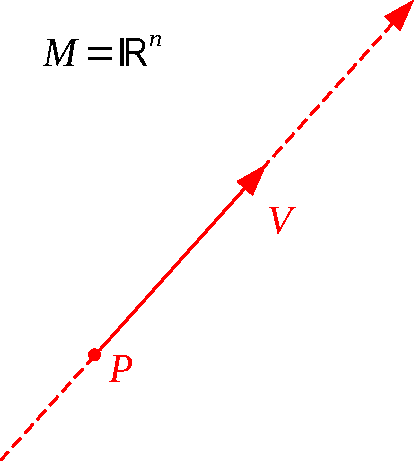
\includegraphics{images/direc_der.pdf}
	\caption[Directional derivative]{Directional derivative}
	\labfig{Dir-deriv}
\end{marginfigure}
\begin{example}\index{Directional derivative}
Let's take a vector $V$, a point $P \in\mathbf{M}$, with $\mathbf{M}=\mathbb{R}^n$, and a function $f:\mathbf{M}\xrightarrow[]{}\mathbb{R}$ such that:
\[
\begin{tikzcd}[cramped, sep=small] 
t &\mapsto & P+tV &\mapsto &f(P+tV)\\
\left(\varepsilon,-\varepsilon\right)\arrow[red, bend right]{rrrr} &\to &\mathbf{M} &\to& \mathbb{R}
\end{tikzcd}
\]
Let us take the direction given by the straight line which pass through $P$ at $t=0$ and goes in the direction $V$. The directional derivative in \textbf{direction} $\mathbf{V}$ at point $P\in\mathbf{M}$ of a function $f:\mathbf{M}\xrightarrow[]{}\mathbb{R}$ is defined as the derivative along this line:
\[
D_v f(P):=\dv{t}f(P+tV)\Bigr|_{\substack{t=0}} \qquad \star
\]
Properties of directional derivative:
\begin{enumerate}
    \item is linear: \ $\begin{cases}
    D_V(f+g)=D_V(f)+D_v(g) \\
    D_V(\lambda g)=\lambda D_v(g)
    \end{cases}
    \forall f,g \in C^{\infty}(\mathbb{R}^n)$
    \item follows the Leibniz rule:\\
    $D_V(f\cdot g)=D_V(f)\cdot g+f\cdot D_V(g) \quad \forall f,g \in\mathbb{C}^{\infty}(\mathbb{R}^n$
\end{enumerate}
In coordinates, we have 
\[
\dv{t}f(P+tV)\Bigr|_{\substack{t=0}}\underset{\mathclap{\tikz \node {$\uparrow$} node [below=1ex] {\footnotesize chain rule};}}{=}\sum_{j=1}^n \frac{\partial f}{\partial x^j}(P) v^j
\]
We can omit the specification of the point and write
\[
D_V f=\underbrace{\left(\sum_{j=1}^n \frac{\partial}{\partial x^j}\right)}_{\mathclap{\text{$1^{\textrm{st}}$ order diff. operator}}}f \qquad \star
\]
\end{example}
This example suggests that we might (alternatively) define tangent vectors at $P \in\mathbf{M}$ as \textbf{directional derivatives} acting on functions $f:\mathbf{M}\supseteq U\xrightarrow[]{}\mathbb{R}$.
\begin{definition}[\href{https://it.wikipedia.org/wiki/Germe_di_funzione}{Germe} - Germ at $P \in\mathbf{M}$]\index{Germ at $P \in\mathbf{M}$}
The \textbf{germ} at $P \in\mathbf{M}$ is the set of locally defined smooth functions defined around $P \in\mathbf{M}$:
\[
\pazocal{F}_p(\mathbf{M})=\left\{f:U_f\xrightarrow{C^\infty}\mathbb{R}\text{ for some \textbf{open} } U_f\subseteq\mathbf{M}\text{ with } P \in U_f\right\}
\]
\end{definition}
Notice if $f$ and $g$ are in $\pazocal{F}_P(\mathbf{M})$ then both $(f+g)$ and $(f\cdot g)$ are in the same set $\pazocal{F}_P(\mathbf{M})$.
\begin{definition}[Tangent vector - algebraic definition]\index{Tangent vector - algebraic definition}
A tangent vector at $P \in\mathbf{M}$ is a map $D_V:\pazocal{F}_P(\mathbf{M})\to\pazocal{F}_p(\mathbf{M})$ which satisfies:
\begin{enumerate}
    \item linear:  $D_V(f+g)=D_V(f)+D_V(g)$
    \item Leibniz $D_V(f\cdot g)=D_V(f)\cdot g+f\cdot D_V(g)$
\end{enumerate}
\end{definition}
\begin{definition}
We define\marginnote{"alg" states for "algebraically defined".}
\(
T_P^{\textrm{alg}}\mathbf{M}=\underset{\mathclap{\tikz \node {$\uparrow$} node [below=1ex] {\footnotesize \textbf{Derivations}: maps that are Linear + Leibniz};}}{\textrm{Der}}\left(\pazocal{F}_P(\mathbf{M})\right)
\)
\end{definition}
%FINE LEZIONE 4 - 11/03/2022
%INIZIO LEZIONE 5 - 17/03/2022
\subsection[Equivalence of viewpoints]{Equivalence of viewpoints}
We now have two viewpoints:
\begin{figure}[H]
	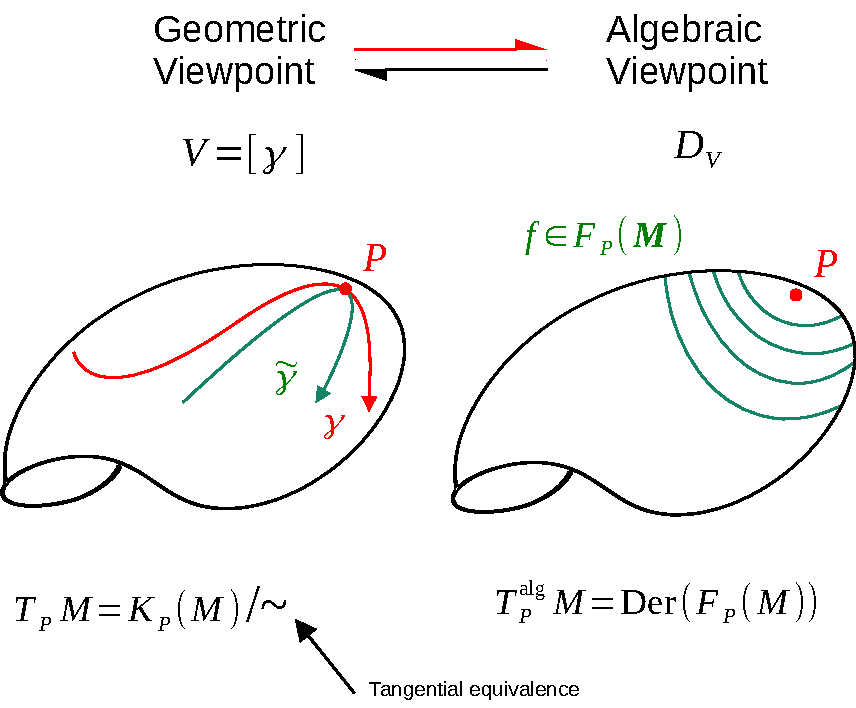
\includegraphics{images/Equivalence_of_viewpoints.pdf}
	\caption[Representation of the two viewpoints]{Representation of the two viewpoints on tangent vector emphasizing their philosophical difference}
	\labfig{equiv-of-view}
\end{figure}
The idea is that we can define a speed and a direction in two ways: either we give course and the velocity we are interested in is the time derivative at time zero of this course (geometric viewpoint\index{Geometric viewpoint}), or we do not give course, but we tell how quickly we go through the level surfaces of any possible test function (algebraic viewpoint\index{Algebraic viewpoint}). This reminds the two viewpoints you have in optics.\\
\underline{Analogy}:\marginnote{Io avrei detto più che altro grazie all'\href{https://en.wikipedia.org/wiki/Eikonal_equation}{equazione dell'eikonale}.}
\[
\text{\parbox{4 cm}{\centering Optical Rays \\[8pt]  {\color{teal} Fermat}}}\underset{\mathclap{\tikz \node {$\uparrow$} node [below=1ex] {\footnotesize \href{https://it.wikipedia.org/wiki/Principio_di_Huygens-Fresnel}{Huygen's theorem}};}}{\simeq}\text{\parbox{4 cm}{\centering wavefront \\[8pt]  {\color{teal} Hamilton}}}
\]
Given a tangent vector $V=\qty[\gamma]\in T_P\mathbf{M}$ we may consider the \textbf{associated directional derivative}, defined starting from a straight line passing through the point $P$ at time $t=0$ and going in the direction $V$. On generic manifolds, there are no straight lines, but the fact that the line is straight is not essential, we could have taken another curve
\[
\left(D_V f\right)_P=\frac{\textrm{d}}{\textrm{d}t}f\Big(\underset{\mathclap{\tikz \node {$\uparrow$} node [below=1ex] {\footnotesize $\gamma(0)=P$} node [below=4ex] {\footnotesize $\qty[\gamma]=V$} ;}}{\gamma}(t)\Big)\Big|_{t=0} \qquad \bigg|\bigg|\quad \star
\]
for $f\in\pazocal{F}_P(\mathbf{M})$.\\
\underline{Ref:} A complete equivalence of viewpoints is in Chapter 2 of \sidecite{Jänich2001}.
\section[Differential of a map]{Differential of a map $\mathbf{M}\xrightarrow{f}\mathbf{N}$}
Let us start with a bit of motivation. We learned in analysis II a very powerful tool in calculus: Taylor's expansion. We would like to have it also for manifolds, but there is a problem, if we have a Taylor's expansion for a map $\mathbb{R}^m\xrightarrow{f}\mathbb{R}^n$
\[
\bigg|\bigg|\quad f(x)-f(x_0)=\underbrace{\left(\textrm{d}f\big|_{x_0}\right)}_{\mathclap{\text{\parbox{4 cm}{\centering Linear \\[-4pt]  operator}}}}\underbrace{\left(x-x_0\right)}_{\mathclap{\text{\parbox{4 cm}{\centering Increment \\[-4pt] in $\mathbb{R}^n$}}}}+o \left(\norm{x-x_0}\right)
\]
In coordinates: \(\left(\textrm{d}f\big|_{\color{red}x_0}\right)^j_{\ l}=\frac{\partial f^j}{\partial x^l}({\color{red} x_0})\).
\begin{figure}[H]
	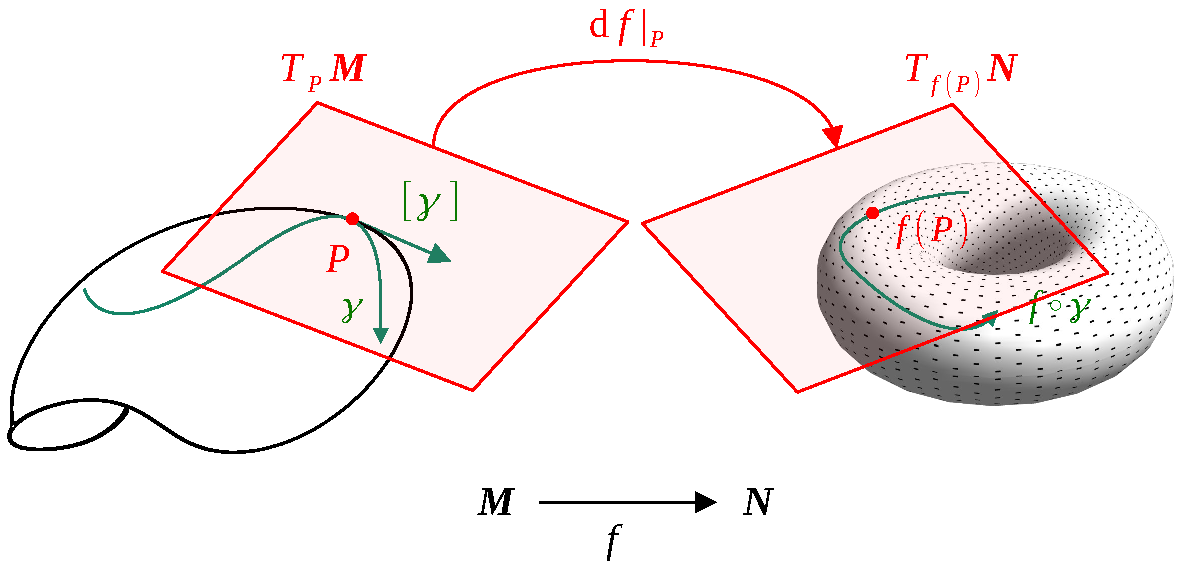
\includegraphics{images/differential_of_a_map.pdf}
	\caption[Differential of a map]{Representation of a map between to manifolds with their tangent linear spaces. $\qty[\gamma]$ is the tangent vector.}
	\labfig{diff-on-a-map}
\end{figure}
We cannot write something like a Taylor's expansion, because we do not have a linear structure.
\begin{definition}[Differential of a map $\mathbf{M}\xrightarrow{f}\mathbf{N}$]
The differential of a map $f:\mathbf{M}\to\mathbf{N}$ is a \textbf{linear map} from $T_P\mathbf{M}$ to $T_{f(P)}\mathbf{N}$ defined by\marginnote{
\begin{kaobox}[frametitle=Remark]
This definition is \textbf{intrinsic}!
\end{kaobox}}
\[
\begin{split}
\textrm{d}f\big|_P : T_P\mathbf{M}& \to  T_{f(P)}\mathbf{N}\\
\qty[\gamma] &\mapsto \qty[f\circ \gamma]
\end{split}
\]
\end{definition}
\begin{example}
Given local charts $(u,\varphi)$ around $P\in\mathbf{M}$ and  $(\nu,\psi)$ around $f(P)\in\mathbf{N}$, compute the \textbf{local expression} of $\textrm{d}f\big|_P$ with respect to this local charts.\marginnote[-3mm]{{\fontencoding{U}\fontfamily{futs}\selectfont\char 66\relax} \underline{Warning}: the local expression of $\textrm{d}f\big|_P$ \textbf{does depend on the local charts!}}
\end{example}
There is an example we can work out in detail
\begin{marginfigure}[8mm]
	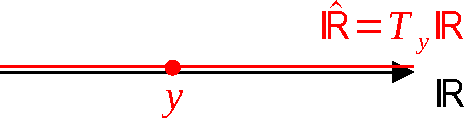
\includegraphics[width=1.2\linewidth]{images/differential_of_a_R_valued_map.pdf}
	\caption[Differential of a $\mathbb{R}$-\textbf{valued} map \(f:\mathbf{M}\to\mathbb{R}\)]{Differential of a $\mathbb{R}$-\textbf{valued} map \(f:\mathbf{M}\to\mathbb{R}\). We put an hat on $\mathbb{R}$ to keep the distinction, we can imagine it is like position space and velocity space, but both are $\mathbb{R}$.}
	\labfig{diff-R-val_map}
\end{marginfigure}
\begin{example}
Differential of a $\mathbb{R}$-\textbf{valued} map \(f:\mathbf{M}\to\mathbb{R}\)
\[
\begin{split}
\textrm{d}f\big|_P : T_P\mathbf{M}& \to  T_{f(P)}\mathbb{R}\cong\mathbb{R}\\
\qty[\gamma] &\mapsto \qty[f\circ \gamma]
\end{split}
\]
\[
\begin{split}
\textrm{d}f\big|_P\left(\qty[\gamma]\right)
&=\qty[f\circ\gamma]=\\
&=\frac{\textrm{d}}{\textrm{d}t}f\circ\gamma(t)\big|_{t=0}=\\
&\overset{\textrm{L.C.}}{=}\sum\frac{\partial f}{\partial x^j}(x_0)\cdot v^j=\\
&=\underbrace{\left(\frac{\partial f}{\partial x^1}(x_0),\dots, \frac{\partial f}{\partial x^n}(x_0)\right)}_{\mathclap{\text{Components of a covector}}}
\begin{pmatrix}
v^1\\
\vdots\\
v^n
\end{pmatrix}
\end{split}
\]
\end{example}
\marginnote[-25mm]{"L.C." = "Local Charts", in this way I can use the chain rule.}
\section{Covectors and Cotangent spaces}
For every $P\in\mathbf{M}$, we know that the tangent space $T_P\mathbf{M}$ is a \textbf{linear space} (or vector space). Since is a linear space, it has a dual we can take. This is the set of linear functionals, all the maps from $T_P\mathbf{M}$ to $\mathbb{R}$ which are linear
\[
\left(T_P\mathbf{M}\right)^\ast=\left\{\alpha:T_P\mathbf{M}\xrightarrow{\textrm{\textbf{linear}}}\mathbb{R}\right\}\equiv T_P^\ast\mathbf{M}
\]
This is a vector space itselfs, with dimension $\dim{T^\ast_P\mathbf{M}}=\dim T_P\mathbf{M}=n$. But there is also a 
\[
\textrm{\underline{Natural coupling:}} \quad \textrm{For } \ V\in T_P\mathbf{M} \ \textrm{ and }\  \alpha\in T_P^\ast\mathbf{M} \ \textrm{ you have }\  \alpha(V)\in\mathbb{R} 
\]
So the covector is a linear functional, it takes a vector and it produces a number. This is like in Geometry I, what is different is that here you can change local charts\marginnote[10mm]{I can write equalities because now they are numbers}
\[
\text{\parbox{2 cm}{\centering local chart \\[-4pt]  $(u,\varphi)$}}\longleftarrow\text{\parbox{2 cm}{\centering intrinsic \\[-4pt]  number}}\longrightarrow\text{\parbox{2 cm}{\centering local chart \\[-4pt] $(\tilde{u},\tilde{\varphi})$}}
\]
\[
\sum_j\alpha_jv^j\qquad =\quad \alpha(V)\quad =\qquad \sum_j\tilde{\alpha}_j\tilde{v}^j
\]
Let us check that what we said is correct: in local chart $(u, \varphi)$ we have $\left\{e_1,\dots,e_n\right\}$
\[
\alpha(V)=\alpha\left(\sum_jv^je_j\right) \underset{\mathclap{\tikz \node {$\uparrow$} node [below=1ex] {\footnotesize $\alpha$ is \textbf{linear}};}}{=} \sum_jv^j\underbrace{\alpha(e_k)}_{=:\alpha_j}= \sum_j v^j\alpha_j
\]
where $\alpha_j$ \textbf{are the components of $\alpha$ w.r.t. $(u,\varphi)$}. To see how the components of a covector transform, we use again\marginnote{So they transform as the coordinate bases}
\[
\text{\parbox{2 cm}{\centering Ricci's \\[-4pt]  rule}}\quad \tilde{\alpha}_{\textcolor{red}{j}}=\sum_{l=1}^n\underbrace{\frac{\partial x^l}{\partial\textcolor{red}{\tilde{x}^j}}}_{\mathclap{\text{Jacobian matrix of the transformation $x(\tilde{x})$}}}\alpha_l \qquad \bigg|\bigg| \quad \text{\parbox{3 cm}{\centering Components of a covector are \textbf{covariant}}}
\]
All the covectors are equal, but some are more equal than others: as we have the coordinate bases in the tangent space, we will have some relavant bases in the cotangent space. The coordinate bases \(\left\{e_1,\dots,e_n\right\}\) is associated to a \textbf{dual bases}\sidenote{We will explain why we use this fancy notation}\index{Dual bases} \(\left\{dx^1,\dots,dx^n\right\}\) defined by this rule
\[
dx^j(e_l)=\delta^j_{\ l}=
\begin{cases}
0 \ & \ \textrm{if } j\neq l\\
1 \ & \ \textrm{if } j= l
\end{cases}
\]
or, equivalently we can say that
\[
dx^j(V)=v^j
\]
The dual bases are \textbf{contravariant}, i.e. transforms
\[
\textrm{d}\tilde{x}^{\textcolor{red}{j}}=\sum_{l=1}^n\underbrace{\frac{\partial \textcolor{red}{\tilde{x}^l}}{\partial{{x}^j}}}_{\mathclap{\text{Jacobian matrix of the transformation $x(\tilde{x})$}}}\textrm{d}x^l \qquad \bigg|\bigg| \quad \text{\parbox{3 cm}{\centering Dual bases are \textbf{contravariant}}}
\]
\section[Tangent and cotangent bundles]{Tangent and cotangent bundles\\\;\;\;\;Fibrato tangente e cotangente}
The tangent \textbf{bundle}\index{Bundle}(\textit{fibrato} in Italian) to a manifold $\mathbf{M}$ is the collection of all the tangent spaces to this manifold, but with additional structure which is the projection on the manifold itself. In more precise words is the \textbf{disjoint union}\sidenote{See the first example on why we use the disjoint union.\\
\href{https://it.wikipedia.org/wiki/Somma_disgiunta}{Disjoint union}: <<In mathematics, a disjoint union (or discriminated union) of a family of sets $(A_{i}:i\in I)$ is a set $A$, often denoted by $\bigsqcup _{i\in I}A_{i}$, with an injection of each $A_{i}$  into $A$, such that the images of these injections form a partition of $A$ (that is, each element of $A$ belongs to exactly one of these images).>> From \href{https://en.wikipedia.org/wiki/Disjoint_union}{Wikipedia}.}
\[
TM := \bigsqcup_{p\in\mathbf{M}}T_PM
\]
equipped with a \textbf{projection} $\Pi: T\mathbf{M}\to\mathbf{M}$ wich sends $T_P\mathbf{M}\ni V \mapsto P\in\mathbf{M}$. If you have a tangent vector to the manifold, it must be a tangent vector to some points and the projector remember to which one is the point. Let us make some non-linear examples.
\begin{marginfigure}[20mm]
	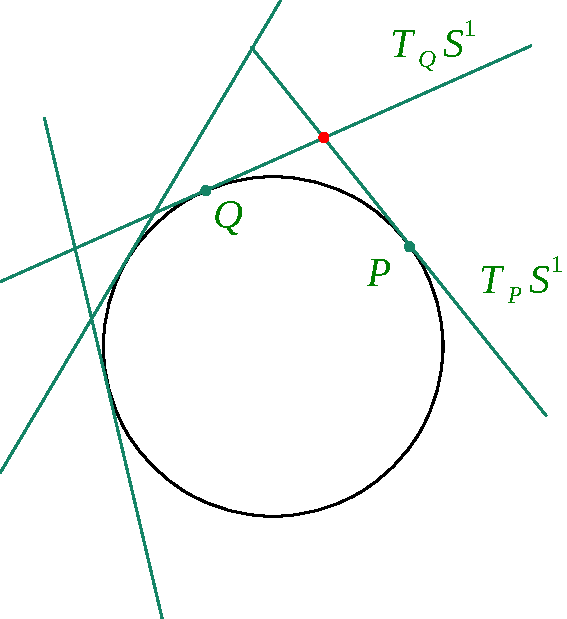
\includegraphics[width=1.2\linewidth]{images/Tangent_bundles.pdf}
	\caption[Tangent bundle]{}
	\labfig{tan-bund}
\end{marginfigure} 
\begin{example}
$\mathbf{M}=S^1$.\\If the manifold is embedded (as in this case \reffig{tan-bund}), there are points which are at the intersection of the two, these have to be counted twice: once as an element of the tangent space to $P$ and once to $Q$. This is the reason why we use the disjoint union. Now we can imagine to take this straight lines and to deform them continuously to put them vertically. It turns out that the tangent space to the circle can be continuously (and even deferentially deformed) into a cylinder:
\[
TS^1\underset{\textrm{diffeo}}{\cong}\underset{\mathclap{\tikz \node {$\uparrow$} node [below=1ex] {\footnotesize cylinder};}}{\pazocal{C}}=S^1\cross \mathbb{R} \quad \textrm{It is \textbf{globally a product!}}
\]
So this particular tangent bundle is a product of a bases times a vector space, this is quite a rare event.
\end{example}
The generic case is that the tangent bundle to a manifold is not the Cartesian product of the manifold times a vector space, as in the next case.
\begin{marginfigure}[-20mm]
	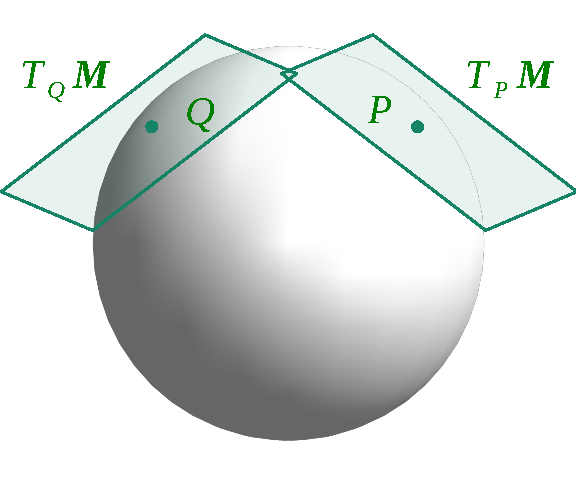
\includegraphics[width=1.2\linewidth]{images/Tangent_bundles_s2.pdf}
	\caption[Tangent bundle $S^2$]{}
	\labfig{tan-bund}
\end{marginfigure} 
\begin{example}
$\mathbf{M}=S^2$.\\
It turns out that the tangent bundle to $S^2$ is not diffeomorphic (it is not even homeomorphic) to the product:
\[
TS^2\underset{\textrm{diffeo}}{\ncong}S^2\cross \mathbb{R}^2 \quad 
\text{\parbox{4 cm}{\centering It is locally a product, \underline{but \textbf{not globally a product!}}}}
\]
This is the generic case. This has to do with the fact that every vector field on the two-sphere (which is smooth and even continuous) must vanish at least at one point \sidecite{arnold2010metodi}. There is no global non-vanish vector field on the two sphere. 
\end{example}
\subsection[Fibre bundles]{\underline{Rem:} Fibre bundles (not required)}\marginnote{A fiber bundle is a generalization of tangent bundle. Tangent and cotangent bundles are special cases of fiber bundles in which the fiber is ??? $u$ di qualcosa.}
Instead of giving the general theory, we will talk about two examples\index{Möbius strip}
\[
\textrm{Cylinder} \quad \textrm{\underline{vs}} \quad \textrm{Möbius strip}
\]
This is the experimental part of the course. Let us take a square, we can do two things:
\begin{itemize}
    \item identify opposite edge with the same orientation and glue them and get a cylinder;
    \item do the opposite operation and what you get is not topologically a cylinder.
\end{itemize}
But these two guys would look locally the same. It means that the Möbius strip is not globally a product, but it is locally a product. 
\begin{figure}[H]
	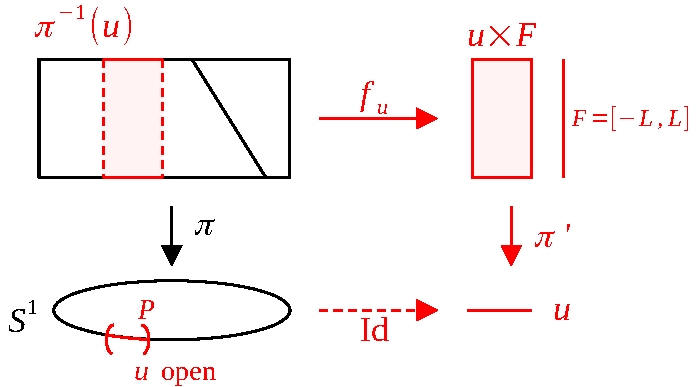
\includegraphics{images/Fiber_bundles.pdf}
	\caption[Fiber Bundles]{$Id=\mathbb{1}$}
	\labfig{fiber-bundles}
\end{figure}
What is important to us is that the Möbius strip is equipped with a projection $\pi$ on the circle. looking at \reffig{fiber-bundles}, the Möbius strip is locally trivial in the sense that for every point $P$, there exits an open $u$ set in the circle $S^1$ such that, if we look to the part of the Möbius strip which is above this $u$, i.e. $\pi^{-1}(u)$, this local portion of the Möbius strip is diffeomorphic to a Cartesian product. This means there exists a function $f_u$ so that the red part of the Möbius strip will be a prodcut of $u$ (the bases) times a fiber (in this case it could be the interval $\left[-L,L\right]$, where $L$ is some number).
Möbius strip is said to be \textbf{locally trivial} in the following sense:\marginnote{In the case of the tangent bundle, the fiber space is a vector space.}\index{Verticality condition}\marginnote[10mm]{The diffeomorphis does not move the points on the bases.}
\[
\forall\ P\in S^1 \quad \exists \ u \textrm{ open with } P\in u \ : \ \exists \textrm{ a map } f_u \textrm{ such that }
\]
\[
\pi^{-1}(u) \xrightarrow[f_u]{\cong} u\times \underset{\mathclap{\tikz \node {$\uparrow$} node [below=1ex] {\footnotesize Fiber space};}}{F} 
\]
\[
\textrm{so that }\ \pi'\circ f_u = \mathbb{1}\circ\pi \quad  \textrm{(\textbf{verticality} condition)}
\]
It means that if we first use $f$ and then project, we get the same thing as first projecting down and then doing nothing (i.e. the identity, it is a technical requirement). However the Möbius strip is \textbf{not a product globally}, i.e.
\[
\textrm{Mö}\ncong S^1 \times F \ \textrm{for any } \ F
\]
Mö is locally trivial (= diffeomorphic to a product). But Mö is \textbf{not globally trivial}, so we say that \textbf{Mö is \underline{non-trivial} fiber bundle}. By letting $L\to\infty$ we obtain examples of trivial/non-trivial \textbf{vector bundles}.
\newline
\paragraph{\underline{Physical relevance}} The math ambient for $T\mathbf{M}$ theories is a (possibly \textbf{non-trivial}) fibre bundle $P\xrightarrow{\pi}\mathbb{M}$ where $\mathbb{M}$ is \textbf{space time} and $P\big|_u=u\times G$ with $G$ a Lie group. ($G=\textrm{U}(1),\textrm{SU}(2),\textrm{SU}(3),\dots$)
\end{document}